\documentclass[1p]{elsarticle_modified}
%\bibliographystyle{elsarticle-num}

%\usepackage[colorlinks]{hyperref}
%\usepackage{abbrmath_seonhwa} %\Abb, \Ascr, \Acal ,\Abf, \Afrak
\usepackage{amsfonts}
\usepackage{amssymb}
\usepackage{amsmath}
\usepackage{amsthm}
\usepackage{scalefnt}
\usepackage{amsbsy}
\usepackage{kotex}
\usepackage{caption}
\usepackage{subfig}
\usepackage{color}
\usepackage{graphicx}
\usepackage{xcolor} %% white, black, red, green, blue, cyan, magenta, yellow
\usepackage{float}
\usepackage{setspace}
\usepackage{hyperref}

\usepackage{tikz}
\usetikzlibrary{arrows}

\usepackage{multirow}
\usepackage{array} % fixed length table
\usepackage{hhline}

%%%%%%%%%%%%%%%%%%%%%
\makeatletter
\renewcommand*\env@matrix[1][\arraystretch]{%
	\edef\arraystretch{#1}%
	\hskip -\arraycolsep
	\let\@ifnextchar\new@ifnextchar
	\array{*\c@MaxMatrixCols c}}
\makeatother %https://tex.stackexchange.com/questions/14071/how-can-i-increase-the-line-spacing-in-a-matrix
%%%%%%%%%%%%%%%

\usepackage[normalem]{ulem}

\newcommand{\msout}[1]{\ifmmode\text{\sout{\ensuremath{#1}}}\else\sout{#1}\fi}
%SOURCE: \msout is \stkout macro in https://tex.stackexchange.com/questions/20609/strikeout-in-math-mode

\newcommand{\cancel}[1]{
	\ifmmode
	{\color{red}\msout{#1}}
	\else
	{\color{red}\sout{#1}}
	\fi
}

\newcommand{\add}[1]{
	{\color{blue}\uwave{#1}}
}

\newcommand{\replace}[2]{
	\ifmmode
	{\color{red}\msout{#1}}{\color{blue}\uwave{#2}}
	\else
	{\color{red}\sout{#1}}{\color{blue}\uwave{#2}}
	\fi
}

\newcommand{\Sol}{\mathcal{S}} %segment
\newcommand{\D}{D} %diagram
\newcommand{\A}{\mathcal{A}} %arc


%%%%%%%%%%%%%%%%%%%%%%%%%%%%%5 test

\def\sl{\operatorname{\textup{SL}}(2,\Cbb)}
\def\psl{\operatorname{\textup{PSL}}(2,\Cbb)}
\def\quan{\mkern 1mu \triangleright \mkern 1mu}

\theoremstyle{definition}
\newtheorem{thm}{Theorem}[section]
\newtheorem{prop}[thm]{Proposition}
\newtheorem{lem}[thm]{Lemma}
\newtheorem{ques}[thm]{Question}
\newtheorem{cor}[thm]{Corollary}
\newtheorem{defn}[thm]{Definition}
\newtheorem{exam}[thm]{Example}
\newtheorem{rmk}[thm]{Remark}
\newtheorem{alg}[thm]{Algorithm}

\newcommand{\I}{\sqrt{-1}}
\begin{document}

%\begin{frontmatter}
%
%\title{Boundary parabolic representations of knots up to 8 crossings}
%
%%% Group authors per affiliation:
%\author{Yunhi Cho} 
%\address{Department of Mathematics, University of Seoul, Seoul, Korea}
%\ead{yhcho@uos.ac.kr}
%
%
%\author{Seonhwa Kim} %\fnref{s_kim}}
%\address{Center for Geometry and Physics, Institute for Basic Science, Pohang, 37673, Korea}
%\ead{ryeona17@ibs.re.kr}
%
%\author{Hyuk Kim}
%\address{Department of Mathematical Sciences, Seoul National University, Seoul 08826, Korea}
%\ead{hyukkim@snu.ac.kr}
%
%\author{Seokbeom Yoon}
%\address{Department of Mathematical Sciences, Seoul National University, Seoul, 08826,  Korea}
%\ead{sbyoon15@snu.ac.kr}
%
%\begin{abstract}
%We find all boundary parabolic representation of knots up to 8 crossings.
%
%\end{abstract}
%\begin{keyword}
%    \MSC[2010] 57M25 
%\end{keyword}
%
%\end{frontmatter}

%\linenumbers
%\tableofcontents
%
\newcommand\colored[1]{\textcolor{white}{\rule[-0.35ex]{0.8em}{1.4ex}}\kern-0.8em\color{red} #1}%
%\newcommand\colored[1]{\textcolor{white}{ #1}\kern-2.17ex	\textcolor{white}{ #1}\kern-1.81ex	\textcolor{white}{ #1}\kern-2.15ex\color{red}#1	}

{\Large $\underline{12n_{0138}~(K12n_{0138})}$}

\setlength{\tabcolsep}{10pt}
\renewcommand{\arraystretch}{1.6}
\vspace{1cm}\begin{tabular}{m{100pt}>{\centering\arraybackslash}m{274pt}}
\multirow{5}{120pt}{
	\centering
	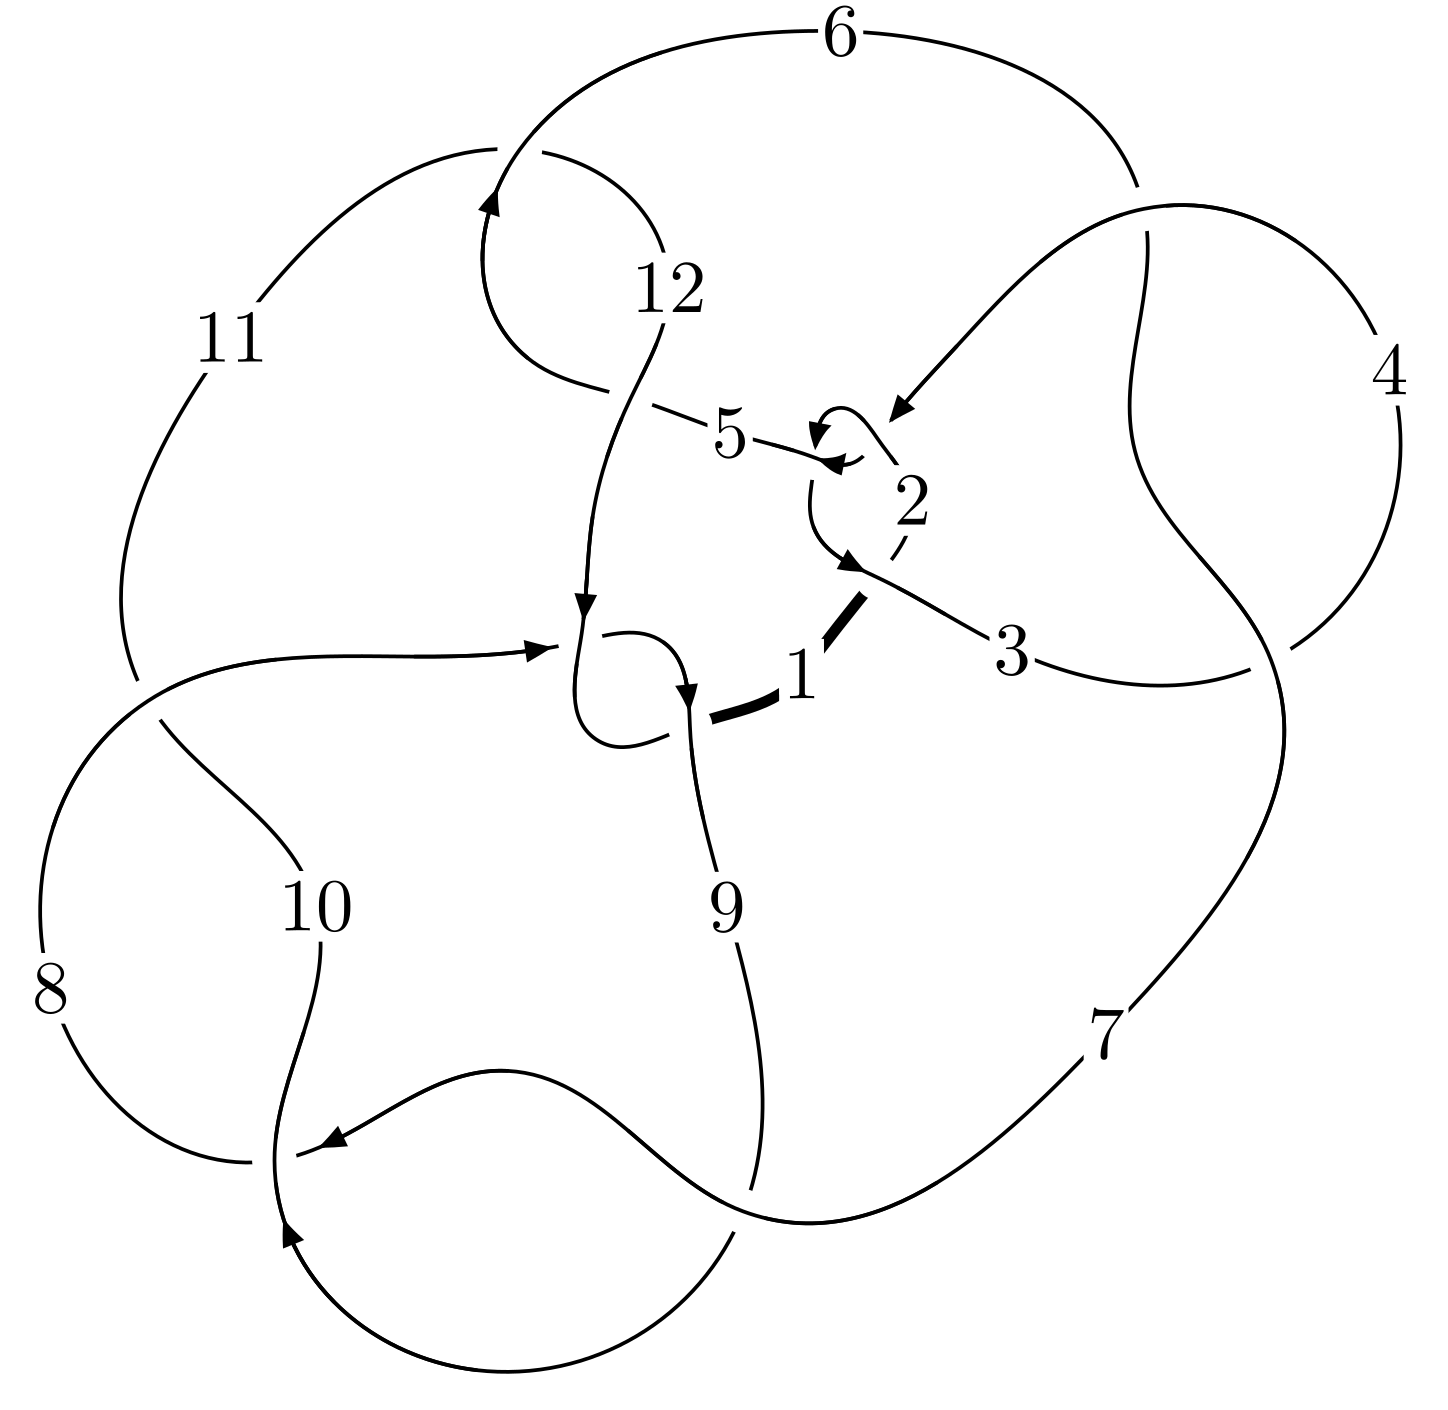
\includegraphics[width=112pt]{../../../GIT/diagram.site/Diagrams/png/2227_12n_0138.png}\\
\ \ \ A knot diagram\footnotemark}&
\allowdisplaybreaks
\textbf{Linearized knot diagam} \\
\cline{2-2}
 &
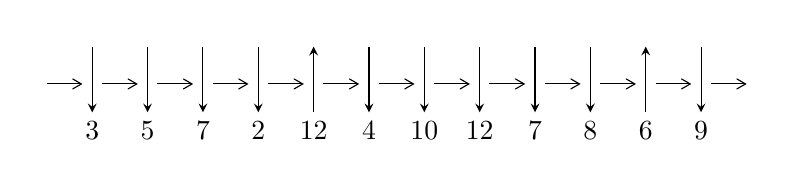
\begin{tikzpicture}[x=20pt, y=17pt]
	% nodes
	\node (C0) at (0, 0) {};
	\node (C1) at (1, 0) {};
	\node (C1U) at (1, +1) {};
	\node (C1D) at (1, -1) {3};

	\node (C2) at (2, 0) {};
	\node (C2U) at (2, +1) {};
	\node (C2D) at (2, -1) {5};

	\node (C3) at (3, 0) {};
	\node (C3U) at (3, +1) {};
	\node (C3D) at (3, -1) {7};

	\node (C4) at (4, 0) {};
	\node (C4U) at (4, +1) {};
	\node (C4D) at (4, -1) {2};

	\node (C5) at (5, 0) {};
	\node (C5U) at (5, +1) {};
	\node (C5D) at (5, -1) {12};

	\node (C6) at (6, 0) {};
	\node (C6U) at (6, +1) {};
	\node (C6D) at (6, -1) {4};

	\node (C7) at (7, 0) {};
	\node (C7U) at (7, +1) {};
	\node (C7D) at (7, -1) {10};

	\node (C8) at (8, 0) {};
	\node (C8U) at (8, +1) {};
	\node (C8D) at (8, -1) {12};

	\node (C9) at (9, 0) {};
	\node (C9U) at (9, +1) {};
	\node (C9D) at (9, -1) {7};

	\node (C10) at (10, 0) {};
	\node (C10U) at (10, +1) {};
	\node (C10D) at (10, -1) {8};

	\node (C11) at (11, 0) {};
	\node (C11U) at (11, +1) {};
	\node (C11D) at (11, -1) {6};

	\node (C12) at (12, 0) {};
	\node (C12U) at (12, +1) {};
	\node (C12D) at (12, -1) {9};
	\node (C13) at (13, 0) {};

	% arrows
	\draw[->,>={angle 60}]
	(C0) edge (C1) (C1) edge (C2) (C2) edge (C3) (C3) edge (C4) (C4) edge (C5) (C5) edge (C6) (C6) edge (C7) (C7) edge (C8) (C8) edge (C9) (C9) edge (C10) (C10) edge (C11) (C11) edge (C12) (C12) edge (C13) ;	\draw[->,>=stealth]
	(C1U) edge (C1D) (C2U) edge (C2D) (C3U) edge (C3D) (C4U) edge (C4D) (C5D) edge (C5U) (C6U) edge (C6D) (C7U) edge (C7D) (C8U) edge (C8D) (C9U) edge (C9D) (C10U) edge (C10D) (C11D) edge (C11U) (C12U) edge (C12D) ;
	\end{tikzpicture} \\
\hhline{~~} \\& 
\textbf{Solving Sequence} \\ \cline{2-2} 
 &
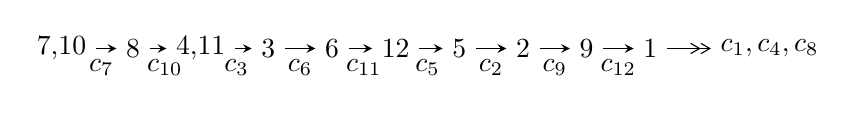
\begin{tikzpicture}[x=23pt, y=7pt]
	% node
	\node (A0) at (-1/8, 0) {7,10};
	\node (A1) at (1, 0) {8};
	\node (A2) at (33/16, 0) {4,11};
	\node (A3) at (25/8, 0) {3};
	\node (A4) at (33/8, 0) {6};
	\node (A5) at (41/8, 0) {12};
	\node (A6) at (49/8, 0) {5};
	\node (A7) at (57/8, 0) {2};
	\node (A8) at (65/8, 0) {9};
	\node (A9) at (73/8, 0) {1};
	\node (C1) at (1/2, -1) {$c_{7}$};
	\node (C2) at (3/2, -1) {$c_{10}$};
	\node (C3) at (21/8, -1) {$c_{3}$};
	\node (C4) at (29/8, -1) {$c_{6}$};
	\node (C5) at (37/8, -1) {$c_{11}$};
	\node (C6) at (45/8, -1) {$c_{5}$};
	\node (C7) at (53/8, -1) {$c_{2}$};
	\node (C8) at (61/8, -1) {$c_{9}$};
	\node (C9) at (69/8, -1) {$c_{12}$};
	\node (A10) at (11, 0) {$c_{1},c_{4},c_{8}$};

	% edge
	\draw[->,>=stealth]	
	(A0) edge (A1) (A1) edge (A2) (A2) edge (A3) (A3) edge (A4) (A4) edge (A5) (A5) edge (A6) (A6) edge (A7) (A7) edge (A8) (A8) edge (A9) ;
	\draw[->>,>={angle 60}]	
	(A9) edge (A10);
\end{tikzpicture} \\ 

\end{tabular} \\

\footnotetext{
The image of knot diagram is generated by the software ``\textbf{Draw programme}" developed by Andrew Bartholomew(\url{http://www.layer8.co.uk/maths/draw/index.htm\#Running-draw}), where we modified some parts for our purpose(\url{https://github.com/CATsTAILs/LinksPainter}).
}\phantom \\ \newline 
\centering \textbf{Ideals for irreducible components\footnotemark of $X_{\text{par}}$} 
 
\begin{align*}
I^u_{1}&=\langle 
1.30613\times10^{24} u^{22}+1.93530\times10^{25} u^{21}+\cdots+3.16864\times10^{26} b-1.61340\times10^{26},\\
\phantom{I^u_{1}}&\phantom{= \langle  }1.48301\times10^{26} u^{22}+2.07464\times10^{27} u^{21}+\cdots+3.16864\times10^{26} a+3.75365\times10^{28},\\
\phantom{I^u_{1}}&\phantom{= \langle  }u^{23}+14 u^{22}+\cdots+247 u-1\rangle \\
I^u_{2}&=\langle 
-676 a^8-5525 a^7+10837 a^6-7123 a^5-92 a^4+4655 a^3-6197 a^2+717 b-295 a+1497,\\
\phantom{I^u_{2}}&\phantom{= \langle  }a^9+7 a^8-25 a^7+34 a^6-25 a^5+9 a^4+5 a^3-6 a^2+1,\;u-1\rangle \\
I^u_{3}&=\langle 
5 a^2 u-3 a^2+12 a u+b-7 a+3 u-1,\;a^3- a^2 u+a^2+3 a u+6 a+3 u+5,\;u^2+u-1\rangle \\
I^u_{4}&=\langle 
b,\;-3 u^2+a-5 u-4,\;u^3+u^2-1\rangle \\
\\
\end{align*}
\raggedright * 4 irreducible components of $\dim_{\mathbb{C}}=0$, with total 41 representations.\\
\footnotetext{All coefficients of polynomials are rational numbers. But the coefficients are sometimes approximated in decimal forms when there is not enough margin.}
\newpage
\renewcommand{\arraystretch}{1}
\centering \section*{I. $I^u_{1}= \langle 1.31\times10^{24} u^{22}+1.94\times10^{25} u^{21}+\cdots+3.17\times10^{26} b-1.61\times10^{26},\;1.48\times10^{26} u^{22}+2.07\times10^{27} u^{21}+\cdots+3.17\times10^{26} a+3.75\times10^{28},\;u^{23}+14 u^{22}+\cdots+247 u-1 \rangle$}
\flushleft \textbf{(i) Arc colorings}\\
\begin{tabular}{m{7pt} m{180pt} m{7pt} m{180pt} }
\flushright $a_{7}=$&$\begin{pmatrix}1\\0\end{pmatrix}$ \\
\flushright $a_{10}=$&$\begin{pmatrix}0\\u\end{pmatrix}$ \\
\flushright $a_{8}=$&$\begin{pmatrix}1\\u^2\end{pmatrix}$ \\
\flushright $a_{4}=$&$\begin{pmatrix}-0.468025 u^{22}-6.54739 u^{21}+\cdots+247.949 u-118.462\\-0.00412206 u^{22}-0.0610765 u^{21}+\cdots+2.33980 u+0.509176\end{pmatrix}$ \\
\flushright $a_{11}=$&$\begin{pmatrix}- u\\- u^3+u\end{pmatrix}$ \\
\flushright $a_{3}=$&$\begin{pmatrix}-0.472147 u^{22}-6.60847 u^{21}+\cdots+250.289 u-117.953\\-0.00412206 u^{22}-0.0610765 u^{21}+\cdots+2.33980 u+0.509176\end{pmatrix}$ \\
\flushright $a_{6}=$&$\begin{pmatrix}0.253629 u^{22}+3.54938 u^{21}+\cdots-137.567 u+62.4798\\8.27189\times10^{-6} u^{22}+0.00149756 u^{21}+\cdots+1.46879 u-0.275118\end{pmatrix}$ \\
\flushright $a_{12}=$&$\begin{pmatrix}0.0618338 u^{22}+0.867080 u^{21}+\cdots-30.7615 u+15.7102\\-0.00140785 u^{22}-0.0182940 u^{21}+\cdots-0.437254 u-0.0618338\end{pmatrix}$ \\
\flushright $a_{5}=$&$\begin{pmatrix}0.273382 u^{22}+3.82624 u^{21}+\cdots-147.561 u+66.4442\\-0.000313866 u^{22}-0.00313831 u^{21}+\cdots+2.38335 u-0.294871\end{pmatrix}$ \\
\flushright $a_{2}=$&$\begin{pmatrix}-0.264797 u^{22}-3.70794 u^{21}+\cdots+143.659 u-63.5528\\0.000313866 u^{22}+0.00313831 u^{21}+\cdots-2.38335 u+0.294871\end{pmatrix}$ \\
\flushright $a_{9}=$&$\begin{pmatrix}u\\u\end{pmatrix}$ \\
\flushright $a_{1}=$&$\begin{pmatrix}0.0632652 u^{22}+0.887387 u^{21}+\cdots-30.6962 u+15.7102\\0.0000236385 u^{22}+0.00201246 u^{21}+\cdots-0.372026 u-0.0618418\end{pmatrix}$\\&\end{tabular}
\flushleft \textbf{(ii) Obstruction class $= -1$}\\~\\
\flushleft \textbf{(iii) Cusp Shapes $= \frac{12439096516079350509692}{1237751551862707466683597} u^{22}+\frac{24959142431741094135677015}{158432198638426555735500416} u^{21}+\cdots+\frac{1416393727615768311794426071}{158432198638426555735500416} u-\frac{1337939601650771137272682937}{158432198638426555735500416}$}\\~\\
\newpage\renewcommand{\arraystretch}{1}
\flushleft \textbf{(iv) u-Polynomials at the component}\newline \\
\begin{tabular}{m{50pt}|m{274pt}}
Crossings & \hspace{64pt}u-Polynomials at each crossing \\
\hline $$\begin{aligned}c_{1}\end{aligned}$$&$\begin{aligned}
&u^{23}+23 u^{22}+\cdots+12783 u+1
\end{aligned}$\\
\hline $$\begin{aligned}c_{2},c_{4}\end{aligned}$$&$\begin{aligned}
&u^{23}-7 u^{22}+\cdots-113 u-1
\end{aligned}$\\
\hline $$\begin{aligned}c_{3},c_{6}\end{aligned}$$&$\begin{aligned}
&u^{23}-4 u^{22}+\cdots-36 u+8
\end{aligned}$\\
\hline $$\begin{aligned}c_{5},c_{11}\end{aligned}$$&$\begin{aligned}
&u^{23}+3 u^{22}+\cdots-32 u-64
\end{aligned}$\\
\hline $$\begin{aligned}c_{7},c_{9},c_{10}\end{aligned}$$&$\begin{aligned}
&u^{23}-14 u^{22}+\cdots+247 u+1
\end{aligned}$\\
\hline $$\begin{aligned}c_{8},c_{12}\end{aligned}$$&$\begin{aligned}
&u^{23}+5 u^{22}+\cdots+4608 u-512
\end{aligned}$\\
\hline
\end{tabular}\\~\\
\newpage\renewcommand{\arraystretch}{1}
\flushleft \textbf{(v) Riley Polynomials at the component}\newline \\
\begin{tabular}{m{50pt}|m{274pt}}
Crossings & \hspace{64pt}Riley Polynomials at each crossing \\
\hline $$\begin{aligned}c_{1}\end{aligned}$$&$\begin{aligned}
&y^{23}-39 y^{22}+\cdots+163240279 y-1
\end{aligned}$\\
\hline $$\begin{aligned}c_{2},c_{4}\end{aligned}$$&$\begin{aligned}
&y^{23}-23 y^{22}+\cdots+12783 y-1
\end{aligned}$\\
\hline $$\begin{aligned}c_{3},c_{6}\end{aligned}$$&$\begin{aligned}
&y^{23}-12 y^{22}+\cdots+7568 y-64
\end{aligned}$\\
\hline $$\begin{aligned}c_{5},c_{11}\end{aligned}$$&$\begin{aligned}
&y^{23}+37 y^{22}+\cdots+234496 y-4096
\end{aligned}$\\
\hline $$\begin{aligned}c_{7},c_{9},c_{10}\end{aligned}$$&$\begin{aligned}
&y^{23}-48 y^{22}+\cdots+59963 y-1
\end{aligned}$\\
\hline $$\begin{aligned}c_{8},c_{12}\end{aligned}$$&$\begin{aligned}
&y^{23}-111 y^{22}+\cdots+71041024 y-262144
\end{aligned}$\\
\hline
\end{tabular}\\~\\
\newpage\flushleft \textbf{(vi) Complex Volumes and Cusp Shapes}
$$\begin{array}{c|c|c}  
\text{Solutions to }I^u_{1}& \I (\text{vol} + \sqrt{-1}CS) & \text{Cusp shape}\\
 \hline 
\begin{aligned}
u &= \phantom{-}0.970382\phantom{ +0.000000I} \\
a &= \phantom{-}8.07238\phantom{ +0.000000I} \\
b &= \phantom{-}0.439625\phantom{ +0.000000I}\end{aligned}
 & -2.87501\phantom{ +0.000000I} & -99.4720\phantom{ +0.000000I} \\ \hline\begin{aligned}
u &= -0.718687 + 0.638413 I \\
a &= \phantom{-}0.403992 - 0.145437 I \\
b &= \phantom{-}0.282905 - 0.561433 I\end{aligned}
 & \phantom{-}1.45854 + 3.25209 I & -3.51442 - 11.82565 I \\ \hline\begin{aligned}
u &= -0.718687 - 0.638413 I \\
a &= \phantom{-}0.403992 + 0.145437 I \\
b &= \phantom{-}0.282905 + 0.561433 I\end{aligned}
 & \phantom{-}1.45854 - 3.25209 I & -3.51442 + 11.82565 I \\ \hline\begin{aligned}
u &= \phantom{-}0.820787 + 0.297606 I \\
a &= \phantom{-}3.29844 - 2.74934 I \\
b &= \phantom{-}0.271589 + 0.441556 I\end{aligned}
 & -2.85899 - 0.09109 I & -11.2448 + 8.7640 I \\ \hline\begin{aligned}
u &= \phantom{-}0.820787 - 0.297606 I \\
a &= \phantom{-}3.29844 + 2.74934 I \\
b &= \phantom{-}0.271589 - 0.441556 I\end{aligned}
 & -2.85899 + 0.09109 I & -11.2448 - 8.7640 I \\ \hline\begin{aligned}
u &= -0.989873 + 0.547667 I \\
a &= -0.262757 - 0.269042 I \\
b &= -0.904186 - 1.051940 I\end{aligned}
 & -5.12106 - 6.15902 I & -10.50715 + 1.63362 I \\ \hline\begin{aligned}
u &= -0.989873 - 0.547667 I \\
a &= -0.262757 + 0.269042 I \\
b &= -0.904186 + 1.051940 I\end{aligned}
 & -5.12106 + 6.15902 I & -10.50715 - 1.63362 I \\ \hline\begin{aligned}
u &= \phantom{-}0.736463\phantom{ +0.000000I} \\
a &= -0.794473\phantom{ +0.000000I} \\
b &= -0.0940545\phantom{ +0.000000I}\end{aligned}
 & -1.10354\phantom{ +0.000000I} & -8.74790\phantom{ +0.000000I} \\ \hline\begin{aligned}
u &= -0.077756 + 0.538901 I \\
a &= -0.928505 + 0.171334 I \\
b &= \phantom{-}0.810706 + 0.505931 I\end{aligned}
 & -0.87687 - 1.52898 I & -6.60742 + 3.54271 I \\ \hline\begin{aligned}
u &= -0.077756 - 0.538901 I \\
a &= -0.928505 - 0.171334 I \\
b &= \phantom{-}0.810706 - 0.505931 I\end{aligned}
 & -0.87687 + 1.52898 I & -6.60742 - 3.54271 I\\
 \hline 
 \end{array}$$\newpage$$\begin{array}{c|c|c}  
\text{Solutions to }I^u_{1}& \I (\text{vol} + \sqrt{-1}CS) & \text{Cusp shape}\\
 \hline 
\begin{aligned}
u &= \phantom{-}0.404196 + 0.182896 I \\
a &= \phantom{-}0.32709 + 2.82080 I \\
b &= \phantom{-}0.273102 - 1.253150 I\end{aligned}
 & \phantom{-}2.20419 + 2.68521 I & \phantom{-}2.70136 + 6.44368 I \\ \hline\begin{aligned}
u &= \phantom{-}0.404196 - 0.182896 I \\
a &= \phantom{-}0.32709 - 2.82080 I \\
b &= \phantom{-}0.273102 + 1.253150 I\end{aligned}
 & \phantom{-}2.20419 - 2.68521 I & \phantom{-}2.70136 - 6.44368 I \\ \hline\begin{aligned}
u &= -1.63114\phantom{ +0.000000I} \\
a &= -1.85070\phantom{ +0.000000I} \\
b &= -0.603575\phantom{ +0.000000I}\end{aligned}
 & -9.92701\phantom{ +0.000000I} & \phantom{-}35.8110\phantom{ +0.000000I} \\ \hline\begin{aligned}
u &= \phantom{-}0.00408400\phantom{ +0.000000I} \\
a &= -117.446\phantom{ +0.000000I} \\
b &= \phantom{-}0.518673\phantom{ +0.000000I}\end{aligned}
 & -1.19404\phantom{ +0.000000I} & -8.40790\phantom{ +0.000000I} \\ \hline\begin{aligned}
u &= -1.89245 + 0.70982 I \\
a &= -1.043110 - 0.396575 I \\
b &= -1.16222 + 1.51464 I\end{aligned}
 & \phantom{-}15.7088 + 13.9110 I & -11.35191 - 5.40734 I \\ \hline\begin{aligned}
u &= -1.89245 - 0.70982 I \\
a &= -1.043110 + 0.396575 I \\
b &= -1.16222 - 1.51464 I\end{aligned}
 & \phantom{-}15.7088 - 13.9110 I & -11.35191 + 5.40734 I \\ \hline\begin{aligned}
u &= -2.26833 + 0.53777 I \\
a &= \phantom{-}0.840120 + 0.152223 I \\
b &= \phantom{-}1.41200 - 1.76863 I\end{aligned}
 & \phantom{-}19.7178 + 6.1351 I & -10.22986 - 1.96379 I \\ \hline\begin{aligned}
u &= -2.26833 - 0.53777 I \\
a &= \phantom{-}0.840120 - 0.152223 I \\
b &= \phantom{-}1.41200 + 1.76863 I\end{aligned}
 & \phantom{-}19.7178 - 6.1351 I & -10.22986 + 1.96379 I \\ \hline\begin{aligned}
u &= \phantom{-}1.99410 + 1.87801 I \\
a &= -0.410446 + 0.386878 I \\
b &= -2.39957 - 0.70874 I\end{aligned}
 & -14.2988 - 3.5584 I & \phantom{-0.000000 } 0 \\ \hline\begin{aligned}
u &= \phantom{-}1.99410 - 1.87801 I \\
a &= -0.410446 - 0.386878 I \\
b &= -2.39957 + 0.70874 I\end{aligned}
 & -14.2988 + 3.5584 I & \phantom{-0.000000 } 0\\
 \hline 
 \end{array}$$\newpage$$\begin{array}{c|c|c}  
\text{Solutions to }I^u_{1}& \I (\text{vol} + \sqrt{-1}CS) & \text{Cusp shape}\\
 \hline 
\begin{aligned}
u &= -2.78866 + 0.30349 I \\
a &= -0.537585 - 0.114355 I \\
b &= -1.97498 - 1.71262 I\end{aligned}
 & \phantom{-}14.2364 + 2.5672 I & \phantom{-0.000000 } 0 \\ \hline\begin{aligned}
u &= -2.78866 - 0.30349 I \\
a &= -0.537585 + 0.114355 I \\
b &= -1.97498 + 1.71262 I\end{aligned}
 & \phantom{-}14.2364 - 2.5672 I & \phantom{-0.000000 } 0 \\ \hline\begin{aligned}
u &= -3.04646\phantom{ +0.000000I} \\
a &= \phantom{-}0.644751\phantom{ +0.000000I} \\
b &= \phantom{-}2.52063\phantom{ +0.000000I}\end{aligned}
 & \phantom{-}18.9120\phantom{ +0.000000I} & \phantom{-0.000000 } 0\\
 \hline 
 \end{array}$$\newpage\newpage\renewcommand{\arraystretch}{1}
\centering \section*{II. $I^u_{2}= \langle -676 a^8+717 b+\cdots-295 a+1497,\;a^9+7 a^8+\cdots-6 a^2+1,\;u-1 \rangle$}
\flushleft \textbf{(i) Arc colorings}\\
\begin{tabular}{m{7pt} m{180pt} m{7pt} m{180pt} }
\flushright $a_{7}=$&$\begin{pmatrix}1\\0\end{pmatrix}$ \\
\flushright $a_{10}=$&$\begin{pmatrix}0\\1\end{pmatrix}$ \\
\flushright $a_{8}=$&$\begin{pmatrix}1\\1\end{pmatrix}$ \\
\flushright $a_{4}=$&$\begin{pmatrix}a\\0.942817 a^{8}+7.70572 a^{7}+\cdots+0.411437 a-2.08787\end{pmatrix}$ \\
\flushright $a_{11}=$&$\begin{pmatrix}-1\\0\end{pmatrix}$ \\
\flushright $a_{3}=$&$\begin{pmatrix}0.942817 a^{8}+7.70572 a^{7}+\cdots+1.41144 a-2.08787\\0.942817 a^{8}+7.70572 a^{7}+\cdots+0.411437 a-2.08787\end{pmatrix}$ \\
\flushright $a_{6}=$&$\begin{pmatrix}-1.10600 a^{8}-8.45607 a^{7}+\cdots+2.08787 a+1.94282\\-2.28870 a^{8}-17.4045 a^{7}+\cdots+4.19107 a+2.41004\end{pmatrix}$ \\
\flushright $a_{12}=$&$\begin{pmatrix}-1.53556 a^{8}-11.8131 a^{7}+\cdots+2.37378 a+0.0794979\\-1.53556 a^{8}-11.8131 a^{7}+\cdots+2.37378 a+0.0794979\end{pmatrix}$ \\
\flushright $a_{5}=$&$\begin{pmatrix}2.51743 a^{8}+18.9149 a^{7}+\cdots-5.17015 a-3.72524\\1.33473 a^{8}+9.96653 a^{7}+\cdots-3.06695 a-3.25802\end{pmatrix}$ \\
\flushright $a_{2}=$&$\begin{pmatrix}2.34589 a^{8}+17.6987 a^{7}+\cdots-4.60251 a-4.32218\\1.33473 a^{8}+9.96653 a^{7}+\cdots-3.06695 a-3.25802\end{pmatrix}$ \\
\flushright $a_{9}=$&$\begin{pmatrix}1\\1\end{pmatrix}$ \\
\flushright $a_{1}=$&$\begin{pmatrix}-1.53556 a^{8}-11.8131 a^{7}+\cdots+2.37378 a+0.0794979\\-1.53556 a^{8}-11.8131 a^{7}+\cdots+2.37378 a+0.0794979\end{pmatrix}$\\&\end{tabular}
\flushleft \textbf{(ii) Obstruction class $= 1$}\\~\\
\flushleft \textbf{(iii) Cusp Shapes $= \frac{10493}{717} a^8+\frac{26713}{239} a^7-\frac{210605}{717} a^6+\frac{75659}{239} a^5-\frac{133631}{717} a^4+\frac{11474}{239} a^3+\frac{50845}{717} a^2-\frac{6563}{239} a-\frac{6150}{239}$}\\~\\
\newpage\renewcommand{\arraystretch}{1}
\flushleft \textbf{(iv) u-Polynomials at the component}\newline \\
\begin{tabular}{m{50pt}|m{274pt}}
Crossings & \hspace{64pt}u-Polynomials at each crossing \\
\hline $$\begin{aligned}c_{1}\end{aligned}$$&$\begin{aligned}
&u^9-5 u^8+12 u^7-15 u^6+9 u^5+u^4-4 u^3+2 u^2+u-1
\end{aligned}$\\
\hline $$\begin{aligned}c_{2}\end{aligned}$$&$\begin{aligned}
&u^9+u^8-2 u^7-3 u^6+u^5+3 u^4+2 u^3- u-1
\end{aligned}$\\
\hline $$\begin{aligned}c_{3}\end{aligned}$$&$\begin{aligned}
&u^9+u^8+2 u^7+u^6+3 u^5+u^4+2 u^3+u-1
\end{aligned}$\\
\hline $$\begin{aligned}c_{4}\end{aligned}$$&$\begin{aligned}
&u^9- u^8-2 u^7+3 u^6+u^5-3 u^4+2 u^3- u+1
\end{aligned}$\\
\hline $$\begin{aligned}c_{5}\end{aligned}$$&$\begin{aligned}
&u^9-3 u^8+8 u^7-13 u^6+17 u^5-17 u^4+12 u^3-6 u^2+u+1
\end{aligned}$\\
\hline $$\begin{aligned}c_{6}\end{aligned}$$&$\begin{aligned}
&u^9- u^8+2 u^7- u^6+3 u^5- u^4+2 u^3+u+1
\end{aligned}$\\
\hline $$\begin{aligned}c_{7}\end{aligned}$$&$\begin{aligned}
&(u-1)^9
\end{aligned}$\\
\hline $$\begin{aligned}c_{8},c_{12}\end{aligned}$$&$\begin{aligned}
&u^9
\end{aligned}$\\
\hline $$\begin{aligned}c_{9},c_{10}\end{aligned}$$&$\begin{aligned}
&(u+1)^9
\end{aligned}$\\
\hline $$\begin{aligned}c_{11}\end{aligned}$$&$\begin{aligned}
&u^9+3 u^8+8 u^7+13 u^6+17 u^5+17 u^4+12 u^3+6 u^2+u-1
\end{aligned}$\\
\hline
\end{tabular}\\~\\
\newpage\renewcommand{\arraystretch}{1}
\flushleft \textbf{(v) Riley Polynomials at the component}\newline \\
\begin{tabular}{m{50pt}|m{274pt}}
Crossings & \hspace{64pt}Riley Polynomials at each crossing \\
\hline $$\begin{aligned}c_{1}\end{aligned}$$&$\begin{aligned}
&y^9- y^8+12 y^7-7 y^6+37 y^5+y^4-10 y^2+5 y-1
\end{aligned}$\\
\hline $$\begin{aligned}c_{2},c_{4}\end{aligned}$$&$\begin{aligned}
&y^9-5 y^8+12 y^7-15 y^6+9 y^5+y^4-4 y^3+2 y^2+y-1
\end{aligned}$\\
\hline $$\begin{aligned}c_{3},c_{6}\end{aligned}$$&$\begin{aligned}
&y^9+3 y^8+8 y^7+13 y^6+17 y^5+17 y^4+12 y^3+6 y^2+y-1
\end{aligned}$\\
\hline $$\begin{aligned}c_{5},c_{11}\end{aligned}$$&$\begin{aligned}
&y^9+7 y^8+20 y^7+25 y^6+5 y^5-15 y^4+22 y^2+13 y-1
\end{aligned}$\\
\hline $$\begin{aligned}c_{7},c_{9},c_{10}\end{aligned}$$&$\begin{aligned}
&(y-1)^9
\end{aligned}$\\
\hline $$\begin{aligned}c_{8},c_{12}\end{aligned}$$&$\begin{aligned}
&y^9
\end{aligned}$\\
\hline
\end{tabular}\\~\\
\newpage\flushleft \textbf{(vi) Complex Volumes and Cusp Shapes}
$$\begin{array}{c|c|c}  
\text{Solutions to }I^u_{2}& \I (\text{vol} + \sqrt{-1}CS) & \text{Cusp shape}\\
 \hline 
\begin{aligned}
u &= \phantom{-}1.00000\phantom{ +0.000000I} \\
a &= \phantom{-}0.162031 + 0.927542 I \\
b &= -0.140343 + 0.966856 I\end{aligned}
 & \phantom{-}0.13850 + 2.09337 I & -6.65973 - 4.50528 I \\ \hline\begin{aligned}
u &= \phantom{-}1.00000\phantom{ +0.000000I} \\
a &= \phantom{-}0.162031 - 0.927542 I \\
b &= -0.140343 - 0.966856 I\end{aligned}
 & \phantom{-}0.13850 - 2.09337 I & -6.65973 + 4.50528 I \\ \hline\begin{aligned}
u &= \phantom{-}1.00000\phantom{ +0.000000I} \\
a &= \phantom{-}0.990590 + 0.515152 I \\
b &= \phantom{-}0.796005 - 0.733148 I\end{aligned}
 & -6.01628 - 1.33617 I & -13.00050 + 1.13735 I \\ \hline\begin{aligned}
u &= \phantom{-}1.00000\phantom{ +0.000000I} \\
a &= \phantom{-}0.990590 - 0.515152 I \\
b &= \phantom{-}0.796005 + 0.733148 I\end{aligned}
 & -6.01628 + 1.33617 I & -13.00050 - 1.13735 I \\ \hline\begin{aligned}
u &= \phantom{-}1.00000\phantom{ +0.000000I} \\
a &= \phantom{-}0.702315 + 0.150499 I \\
b &= \phantom{-}0.728966 + 0.986295 I\end{aligned}
 & -5.24306 - 7.08493 I & -11.6081 + 10.4867 I \\ \hline\begin{aligned}
u &= \phantom{-}1.00000\phantom{ +0.000000I} \\
a &= \phantom{-}0.702315 - 0.150499 I \\
b &= \phantom{-}0.728966 - 0.986295 I\end{aligned}
 & -5.24306 + 7.08493 I & -11.6081 - 10.4867 I \\ \hline\begin{aligned}
u &= \phantom{-}1.00000\phantom{ +0.000000I} \\
a &= -0.405386 + 0.113252 I \\
b &= -0.628449 - 0.875112 I\end{aligned}
 & -2.26187 - 2.45442 I & -9.69685 + 4.13179 I \\ \hline\begin{aligned}
u &= \phantom{-}1.00000\phantom{ +0.000000I} \\
a &= -0.405386 - 0.113252 I \\
b &= -0.628449 + 0.875112 I\end{aligned}
 & -2.26187 + 2.45442 I & -9.69685 - 4.13179 I \\ \hline\begin{aligned}
u &= \phantom{-}1.00000\phantom{ +0.000000I} \\
a &= -9.89910\phantom{ +0.000000I} \\
b &= -0.512358\phantom{ +0.000000I}\end{aligned}
 & -2.84338\phantom{ +0.000000I} & \phantom{-}193.930\phantom{ +0.000000I}\\
 \hline 
 \end{array}$$\newpage\newpage\renewcommand{\arraystretch}{1}
\centering \section*{III. $I^u_{3}= \langle 5 a^2 u-3 a^2+12 a u+b-7 a+3 u-1,\;a^3- a^2 u+a^2+3 a u+6 a+3 u+5,\;u^2+u-1 \rangle$}
\flushleft \textbf{(i) Arc colorings}\\
\begin{tabular}{m{7pt} m{180pt} m{7pt} m{180pt} }
\flushright $a_{7}=$&$\begin{pmatrix}1\\0\end{pmatrix}$ \\
\flushright $a_{10}=$&$\begin{pmatrix}0\\u\end{pmatrix}$ \\
\flushright $a_{8}=$&$\begin{pmatrix}1\\- u+1\end{pmatrix}$ \\
\flushright $a_{4}=$&$\begin{pmatrix}a\\-5 a^2 u+3 a^2-12 a u+7 a-3 u+1\end{pmatrix}$ \\
\flushright $a_{11}=$&$\begin{pmatrix}- u\\- u+1\end{pmatrix}$ \\
\flushright $a_{3}=$&$\begin{pmatrix}-5 a^2 u+3 a^2-12 a u+8 a-3 u+1\\-5 a^2 u+3 a^2-12 a u+7 a-3 u+1\end{pmatrix}$ \\
\flushright $a_{6}=$&$\begin{pmatrix}- a^2 u+a^2-3 a u+2 a- u+1\\-2 a^2 u+a^2-5 a u+3 a-2 u+1\end{pmatrix}$ \\
\flushright $a_{12}=$&$\begin{pmatrix}- u\\- u+1\end{pmatrix}$ \\
\flushright $a_{5}=$&$\begin{pmatrix}- a^2 u+a^2-3 a u+2 a- u+1\\-2 a^2 u+a^2-5 a u+3 a-2 u+1\end{pmatrix}$ \\
\flushright $a_{2}=$&$\begin{pmatrix}-3 a^2 u+2 a^2-8 a u+5 a-3 u\\-2 a^2 u+a^2-5 a u+3 a-2 u+1\end{pmatrix}$ \\
\flushright $a_{9}=$&$\begin{pmatrix}u\\u\end{pmatrix}$ \\
\flushright $a_{1}=$&$\begin{pmatrix}-1\\0\end{pmatrix}$\\&\end{tabular}
\flushleft \textbf{(ii) Obstruction class $= 1$}\\~\\
\flushleft \textbf{(iii) Cusp Shapes $= 17 a^2 u-9 a^2+24 a u-10 a+3 u-18$}\\~\\
\newpage\renewcommand{\arraystretch}{1}
\flushleft \textbf{(iv) u-Polynomials at the component}\newline \\
\begin{tabular}{m{50pt}|m{274pt}}
Crossings & \hspace{64pt}u-Polynomials at each crossing \\
\hline $$\begin{aligned}c_{1},c_{3}\end{aligned}$$&$\begin{aligned}
&(u^3- u^2+2 u-1)^2
\end{aligned}$\\
\hline $$\begin{aligned}c_{2}\end{aligned}$$&$\begin{aligned}
&(u^3+u^2-1)^2
\end{aligned}$\\
\hline $$\begin{aligned}c_{4}\end{aligned}$$&$\begin{aligned}
&(u^3- u^2+1)^2
\end{aligned}$\\
\hline $$\begin{aligned}c_{5},c_{11}\end{aligned}$$&$\begin{aligned}
&u^6
\end{aligned}$\\
\hline $$\begin{aligned}c_{6}\end{aligned}$$&$\begin{aligned}
&(u^3+u^2+2 u+1)^2
\end{aligned}$\\
\hline $$\begin{aligned}c_{7},c_{8}\end{aligned}$$&$\begin{aligned}
&(u^2+u-1)^3
\end{aligned}$\\
\hline $$\begin{aligned}c_{9},c_{10},c_{12}\end{aligned}$$&$\begin{aligned}
&(u^2- u-1)^3
\end{aligned}$\\
\hline
\end{tabular}\\~\\
\newpage\renewcommand{\arraystretch}{1}
\flushleft \textbf{(v) Riley Polynomials at the component}\newline \\
\begin{tabular}{m{50pt}|m{274pt}}
Crossings & \hspace{64pt}Riley Polynomials at each crossing \\
\hline $$\begin{aligned}c_{1},c_{3},c_{6}\end{aligned}$$&$\begin{aligned}
&(y^3+3 y^2+2 y-1)^2
\end{aligned}$\\
\hline $$\begin{aligned}c_{2},c_{4}\end{aligned}$$&$\begin{aligned}
&(y^3- y^2+2 y-1)^2
\end{aligned}$\\
\hline $$\begin{aligned}c_{5},c_{11}\end{aligned}$$&$\begin{aligned}
&y^6
\end{aligned}$\\
\hline $$\begin{aligned}c_{7},c_{8},c_{9}\\c_{10},c_{12}\end{aligned}$$&$\begin{aligned}
&(y^2-3 y+1)^3
\end{aligned}$\\
\hline
\end{tabular}\\~\\
\newpage\flushleft \textbf{(vi) Complex Volumes and Cusp Shapes}
$$\begin{array}{c|c|c}  
\text{Solutions to }I^u_{3}& \I (\text{vol} + \sqrt{-1}CS) & \text{Cusp shape}\\
 \hline 
\begin{aligned}
u &= \phantom{-}0.618034\phantom{ +0.000000I} \\
a &= -0.832857\phantom{ +0.000000I} \\
b &= -0.569840\phantom{ +0.000000I}\end{aligned}
 & -2.10041\phantom{ +0.000000I} & -19.1260\phantom{ +0.000000I} \\ \hline\begin{aligned}
u &= \phantom{-}0.618034\phantom{ +0.000000I} \\
a &= \phantom{-}0.22545 + 2.85986 I \\
b &= -0.215080 - 1.307140 I\end{aligned}
 & \phantom{-}2.03717 - 2.82812 I & -27.3018 + 15.7639 I \\ \hline\begin{aligned}
u &= \phantom{-}0.618034\phantom{ +0.000000I} \\
a &= \phantom{-}0.22545 - 2.85986 I \\
b &= -0.215080 + 1.307140 I\end{aligned}
 & \phantom{-}2.03717 + 2.82812 I & -27.3018 - 15.7639 I \\ \hline\begin{aligned}
u &= -1.61803\phantom{ +0.000000I} \\
a &= -0.255488 + 0.062996 I \\
b &= -0.215080 + 1.307140 I\end{aligned}
 & -5.85852 + 2.82812 I & -12.61597 - 1.90115 I \\ \hline\begin{aligned}
u &= -1.61803\phantom{ +0.000000I} \\
a &= -0.255488 - 0.062996 I \\
b &= -0.215080 - 1.307140 I\end{aligned}
 & -5.85852 - 2.82812 I & -12.61597 + 1.90115 I \\ \hline\begin{aligned}
u &= -1.61803\phantom{ +0.000000I} \\
a &= -2.10706\phantom{ +0.000000I} \\
b &= -0.569840\phantom{ +0.000000I}\end{aligned}
 & -9.99610\phantom{ +0.000000I} & -82.0390\phantom{ +0.000000I}\\
 \hline 
 \end{array}$$\newpage\newpage\renewcommand{\arraystretch}{1}
\centering \section*{IV. $I^u_{4}= \langle b,\;-3 u^2+a-5 u-4,\;u^3+u^2-1 \rangle$}
\flushleft \textbf{(i) Arc colorings}\\
\begin{tabular}{m{7pt} m{180pt} m{7pt} m{180pt} }
\flushright $a_{7}=$&$\begin{pmatrix}1\\0\end{pmatrix}$ \\
\flushright $a_{10}=$&$\begin{pmatrix}0\\u\end{pmatrix}$ \\
\flushright $a_{8}=$&$\begin{pmatrix}1\\u^2\end{pmatrix}$ \\
\flushright $a_{4}=$&$\begin{pmatrix}3 u^2+5 u+4\\0\end{pmatrix}$ \\
\flushright $a_{11}=$&$\begin{pmatrix}- u\\u^2+u-1\end{pmatrix}$ \\
\flushright $a_{3}=$&$\begin{pmatrix}3 u^2+5 u+4\\0\end{pmatrix}$ \\
\flushright $a_{6}=$&$\begin{pmatrix}1\\0\end{pmatrix}$ \\
\flushright $a_{12}=$&$\begin{pmatrix}u^2-1\\u^2+u-1\end{pmatrix}$ \\
\flushright $a_{5}=$&$\begin{pmatrix}-2 u^2+2\\-2 u^2- u+2\end{pmatrix}$ \\
\flushright $a_{2}=$&$\begin{pmatrix}5 u^2+5 u+2\\2 u^2+u-2\end{pmatrix}$ \\
\flushright $a_{9}=$&$\begin{pmatrix}u\\u\end{pmatrix}$ \\
\flushright $a_{1}=$&$\begin{pmatrix}2 u^2-2\\2 u^2+u-2\end{pmatrix}$\\&\end{tabular}
\flushleft \textbf{(ii) Obstruction class $= 1$}\\~\\
\flushleft \textbf{(iii) Cusp Shapes $= 21 u^2+45 u+27$}\\~\\
\newpage\renewcommand{\arraystretch}{1}
\flushleft \textbf{(iv) u-Polynomials at the component}\newline \\
\begin{tabular}{m{50pt}|m{274pt}}
Crossings & \hspace{64pt}u-Polynomials at each crossing \\
\hline $$\begin{aligned}c_{1},c_{2}\end{aligned}$$&$\begin{aligned}
&(u-1)^3
\end{aligned}$\\
\hline $$\begin{aligned}c_{3},c_{6}\end{aligned}$$&$\begin{aligned}
&u^3
\end{aligned}$\\
\hline $$\begin{aligned}c_{4}\end{aligned}$$&$\begin{aligned}
&(u+1)^3
\end{aligned}$\\
\hline $$\begin{aligned}c_{5}\end{aligned}$$&$\begin{aligned}
&u^3+3 u^2+2 u-1
\end{aligned}$\\
\hline $$\begin{aligned}c_{7}\end{aligned}$$&$\begin{aligned}
&u^3+u^2-1
\end{aligned}$\\
\hline $$\begin{aligned}c_{8}\end{aligned}$$&$\begin{aligned}
&u^3- u^2+2 u-1
\end{aligned}$\\
\hline $$\begin{aligned}c_{9},c_{10}\end{aligned}$$&$\begin{aligned}
&u^3- u^2+1
\end{aligned}$\\
\hline $$\begin{aligned}c_{11}\end{aligned}$$&$\begin{aligned}
&u^3-3 u^2+2 u+1
\end{aligned}$\\
\hline $$\begin{aligned}c_{12}\end{aligned}$$&$\begin{aligned}
&u^3+u^2+2 u+1
\end{aligned}$\\
\hline
\end{tabular}\\~\\
\newpage\renewcommand{\arraystretch}{1}
\flushleft \textbf{(v) Riley Polynomials at the component}\newline \\
\begin{tabular}{m{50pt}|m{274pt}}
Crossings & \hspace{64pt}Riley Polynomials at each crossing \\
\hline $$\begin{aligned}c_{1},c_{2},c_{4}\end{aligned}$$&$\begin{aligned}
&(y-1)^3
\end{aligned}$\\
\hline $$\begin{aligned}c_{3},c_{6}\end{aligned}$$&$\begin{aligned}
&y^3
\end{aligned}$\\
\hline $$\begin{aligned}c_{5},c_{11}\end{aligned}$$&$\begin{aligned}
&y^3-5 y^2+10 y-1
\end{aligned}$\\
\hline $$\begin{aligned}c_{7},c_{9},c_{10}\end{aligned}$$&$\begin{aligned}
&y^3- y^2+2 y-1
\end{aligned}$\\
\hline $$\begin{aligned}c_{8},c_{12}\end{aligned}$$&$\begin{aligned}
&y^3+3 y^2+2 y-1
\end{aligned}$\\
\hline
\end{tabular}\\~\\
\newpage\flushleft \textbf{(vi) Complex Volumes and Cusp Shapes}
$$\begin{array}{c|c|c}  
\text{Solutions to }I^u_{4}& \I (\text{vol} + \sqrt{-1}CS) & \text{Cusp shape}\\
 \hline 
\begin{aligned}
u &= -0.877439 + 0.744862 I \\
a &= \phantom{-}0.258045 - 0.197115 I \\
b &= \phantom{-0.000000 } 0\end{aligned}
 & \phantom{-}1.37919 + 2.82812 I & -7.96807 + 6.06881 I \\ \hline\begin{aligned}
u &= -0.877439 - 0.744862 I \\
a &= \phantom{-}0.258045 + 0.197115 I \\
b &= \phantom{-0.000000 } 0\end{aligned}
 & \phantom{-}1.37919 - 2.82812 I & -7.96807 - 6.06881 I \\ \hline\begin{aligned}
u &= \phantom{-}0.754878\phantom{ +0.000000I} \\
a &= \phantom{-}9.48391\phantom{ +0.000000I} \\
b &= \phantom{-0.000000 } 0\end{aligned}
 & -2.75839\phantom{ +0.000000I} & \phantom{-}72.9360\phantom{ +0.000000I}\\
 \hline 
 \end{array}$$\newpage
\newpage\renewcommand{\arraystretch}{1}
\centering \section*{ V. u-Polynomials}
\begin{tabular}{m{50pt}|m{274pt}}
Crossings & \hspace{64pt}u-Polynomials at each crossing \\
\hline $$\begin{aligned}c_{1}\end{aligned}$$&$\begin{aligned}
&(u-1)^3(u^3- u^2+2 u-1)^2\\
&\cdot(u^9-5 u^8+12 u^7-15 u^6+9 u^5+u^4-4 u^3+2 u^2+u-1)\\
&\cdot(u^{23}+23 u^{22}+\cdots+12783 u+1)
\end{aligned}$\\
\hline $$\begin{aligned}c_{2}\end{aligned}$$&$\begin{aligned}
&(u-1)^3(u^3+u^2-1)^2(u^9+u^8-2 u^7-3 u^6+u^5+3 u^4+2 u^3- u-1)\\
&\cdot(u^{23}-7 u^{22}+\cdots-113 u-1)
\end{aligned}$\\
\hline $$\begin{aligned}c_{3}\end{aligned}$$&$\begin{aligned}
&u^3(u^3- u^2+2 u-1)^2(u^9+u^8+2 u^7+u^6+3 u^5+u^4+2 u^3+u-1)\\
&\cdot(u^{23}-4 u^{22}+\cdots-36 u+8)
\end{aligned}$\\
\hline $$\begin{aligned}c_{4}\end{aligned}$$&$\begin{aligned}
&(u+1)^3(u^3- u^2+1)^2(u^9- u^8-2 u^7+3 u^6+u^5-3 u^4+2 u^3- u+1)\\
&\cdot(u^{23}-7 u^{22}+\cdots-113 u-1)
\end{aligned}$\\
\hline $$\begin{aligned}c_{5}\end{aligned}$$&$\begin{aligned}
&u^6(u^3+3 u^2+2 u-1)\\
&\cdot(u^9-3 u^8+8 u^7-13 u^6+17 u^5-17 u^4+12 u^3-6 u^2+u+1)\\
&\cdot(u^{23}+3 u^{22}+\cdots-32 u-64)
\end{aligned}$\\
\hline $$\begin{aligned}c_{6}\end{aligned}$$&$\begin{aligned}
&u^3(u^3+u^2+2 u+1)^2(u^9- u^8+2 u^7- u^6+3 u^5- u^4+2 u^3+u+1)\\
&\cdot(u^{23}-4 u^{22}+\cdots-36 u+8)
\end{aligned}$\\
\hline $$\begin{aligned}c_{7}\end{aligned}$$&$\begin{aligned}
&((u-1)^9)(u^2+u-1)^3(u^3+u^2-1)(u^{23}-14 u^{22}+\cdots+247 u+1)
\end{aligned}$\\
\hline $$\begin{aligned}c_{8}\end{aligned}$$&$\begin{aligned}
&u^9(u^2+u-1)^3(u^3- u^2+2 u-1)(u^{23}+5 u^{22}+\cdots+4608 u-512)
\end{aligned}$\\
\hline $$\begin{aligned}c_{9},c_{10}\end{aligned}$$&$\begin{aligned}
&((u+1)^9)(u^2- u-1)^3(u^3- u^2+1)(u^{23}-14 u^{22}+\cdots+247 u+1)
\end{aligned}$\\
\hline $$\begin{aligned}c_{11}\end{aligned}$$&$\begin{aligned}
&u^6(u^3-3 u^2+2 u+1)\\
&\cdot(u^9+3 u^8+8 u^7+13 u^6+17 u^5+17 u^4+12 u^3+6 u^2+u-1)\\
&\cdot(u^{23}+3 u^{22}+\cdots-32 u-64)
\end{aligned}$\\
\hline $$\begin{aligned}c_{12}\end{aligned}$$&$\begin{aligned}
&u^9(u^2- u-1)^3(u^3+u^2+2 u+1)(u^{23}+5 u^{22}+\cdots+4608 u-512)
\end{aligned}$\\
\hline
\end{tabular}\newpage\renewcommand{\arraystretch}{1}
\centering \section*{ VI. Riley Polynomials}
\begin{tabular}{m{50pt}|m{274pt}}
Crossings & \hspace{64pt}Riley Polynomials at each crossing \\
\hline $$\begin{aligned}c_{1}\end{aligned}$$&$\begin{aligned}
&(y-1)^3(y^3+3 y^2+2 y-1)^2\\
&\cdot(y^9- y^8+12 y^7-7 y^6+37 y^5+y^4-10 y^2+5 y-1)\\
&\cdot(y^{23}-39 y^{22}+\cdots+163240279 y-1)
\end{aligned}$\\
\hline $$\begin{aligned}c_{2},c_{4}\end{aligned}$$&$\begin{aligned}
&(y-1)^3(y^3- y^2+2 y-1)^2\\
&\cdot(y^9-5 y^8+12 y^7-15 y^6+9 y^5+y^4-4 y^3+2 y^2+y-1)\\
&\cdot(y^{23}-23 y^{22}+\cdots+12783 y-1)
\end{aligned}$\\
\hline $$\begin{aligned}c_{3},c_{6}\end{aligned}$$&$\begin{aligned}
&y^3(y^3+3 y^2+2 y-1)^2\\
&\cdot(y^9+3 y^8+8 y^7+13 y^6+17 y^5+17 y^4+12 y^3+6 y^2+y-1)\\
&\cdot(y^{23}-12 y^{22}+\cdots+7568 y-64)
\end{aligned}$\\
\hline $$\begin{aligned}c_{5},c_{11}\end{aligned}$$&$\begin{aligned}
&y^6(y^3-5 y^2+10 y-1)\\
&\cdot(y^9+7 y^8+20 y^7+25 y^6+5 y^5-15 y^4+22 y^2+13 y-1)\\
&\cdot(y^{23}+37 y^{22}+\cdots+234496 y-4096)
\end{aligned}$\\
\hline $$\begin{aligned}c_{7},c_{9},c_{10}\end{aligned}$$&$\begin{aligned}
&(y-1)^9(y^2-3 y+1)^3(y^3- y^2+2 y-1)\\
&\cdot(y^{23}-48 y^{22}+\cdots+59963 y-1)
\end{aligned}$\\
\hline $$\begin{aligned}c_{8},c_{12}\end{aligned}$$&$\begin{aligned}
&y^9(y^2-3 y+1)^3(y^3+3 y^2+2 y-1)\\
&\cdot(y^{23}-111 y^{22}+\cdots+71041024 y-262144)
\end{aligned}$\\
\hline
\end{tabular}
\vskip 2pc
\end{document}